\documentclass[a4paper,11pt]{article}
\usepackage{amsmath,amsthm,amsfonts,amssymb,amscd,amstext,vmargin,graphics,graphicx,tabularx,multicol} 
\usepackage[francais]{babel}
\usepackage[utf8]{inputenc}  
\usepackage[T1]{fontenc} 
\usepackage{pstricks-add,tikz,tkz-tab,variations}
\usepackage[autolanguage,np]{numprint} 

\setmarginsrb{1.5cm}{0.5cm}{1cm}{0.5cm}{0cm}{0cm}{0cm}{0cm} %Gauche, haut, droite, haut
\newcounter{numexo}
\newcommand{\exo}[1]{\stepcounter{numexo}\noindent{\bf Exercice~\thenumexo} : \marginpar{\hfill /#1}}
\reversemarginpar


\newcounter{enumtabi}
\newcounter{enumtaba}
\newcommand{\q}{\stepcounter{enumtabi} \theenumtabi.  }
\newcommand{\qa}{\stepcounter{enumtaba} (\alph{enumtaba}) }
\newcommand{\initq}{\setcounter{enumtabi}{0}}
\newcommand{\initqa}{\setcounter{enumtaba}{0}}

\newcommand{\be}{\begin{enumerate}}
\newcommand{\ee}{\end{enumerate}}
\newcommand{\bi}{\begin{itemize}}
\newcommand{\ei}{\end{itemize}}
\newcommand{\bp}{\begin{pspicture*}}
\newcommand{\ep}{\end{pspicture*}}
\newcommand{\bt}{\begin{tabular}}
\newcommand{\et}{\end{tabular}}
\renewcommand{\tabularxcolumn}[1]{>{\centering}m{#1}} %(colonne m{} centrée, au lieu de p par défault) 
\newcommand{\tnl}{\tabularnewline}

\newcommand{\bmul}[1]{\begin{multicols}{#1}}
\newcommand{\emul}{\end{multicols}}

\newcommand{\trait}{\noindent \rule{\linewidth}{0.2mm}}
\newcommand{\hs}[1]{\hspace{#1}}
\newcommand{\vs}[1]{\vspace{#1}}

\newcommand{\N}{\mathbb{N}}
\newcommand{\Z}{\mathbb{Z}}
\newcommand{\R}{\mathbb{R}}
\newcommand{\C}{\mathbb{C}}
\newcommand{\Dcal}{\mathcal{D}}
\newcommand{\Ccal}{\mathcal{C}}
\newcommand{\mc}{\mathcal}

\newcommand{\vect}[1]{\overrightarrow{#1}}
\newcommand{\ds}{\displaystyle}
\newcommand{\eq}{\quad \Leftrightarrow \quad}
\newcommand{\vecti}{\vec{\imath}}
\newcommand{\vectj}{\vec{\jmath}}
\newcommand{\Oij}{(O;\vec{\imath}, \vec{\jmath})}
\newcommand{\OIJ}{(O;I,J)}


\newcommand{\reponse}[1][1]{%
\multido{}{#1}{\makebox[\linewidth]{\rule[0pt]{0pt}{20pt}\dotfill}
}}

\newcommand{\titre}[5] 
% #1: titre #2: haut gauche #3: bas gauche #4: haut droite #5: bas droite
{
\noindent #2 \hfill #4 \\
#3 \hfill #5

\vspace{-1.6cm}

\begin{center}\rule{6cm}{0.5mm}\end{center}
\vspace{0.2cm}
\begin{center}{\large{\textbf{#1}}}\end{center}
\begin{center}\rule{6cm}{0.5mm}\end{center}
}



\begin{document}
\pagestyle{empty}

\begin{center}
\begin{Large}
\textbf{Séance d'Ap : Les statistiques}\\
\textit{(fréquences, moyenne)}
\end{Large}
\end{center}

\vspace*{0.2cm}

\setlength{\fboxrule}{2pt}
\begin{flushleft}
\framebox{\begin{minipage}{\linewidth}

\vspace*{0.5cm}

\underline{\textbf{Rappels de cours}}\\

\textbf{Effectif total :} nombre de valeurs de la série.\\



\textbf{Effectif d'une valeur :} nombre de fois où la valeur apparaît dans la série.\\

\textbf{Fréquence (en $\%$) :} $f=\dfrac{\text{Effectif de la valeur}}{\text{Effectif total}} (\times 100)$ \\
\textit{(Exemple : Si une valeur apparaît 4 fois sur les 30 valeurs au total, on calcule $f=\dfrac{4}{30} \approx 13,3 \%$ )}\\

\textbf{Calcul d'une moyenne pondérée:} \\

\begin{tabular}{|c|c|c|c|c|}
\hline 
\textbf{Notes} & 8 & 11 & 13 & 17 \\ 
\hline 
\textbf{Coefficients} & 4 & 1 & 2 & 3 \\ 
\hline 
\end{tabular} \hspace*{1cm} $M = \dfrac{(4 \times 8) + (1 \times 11) + (2 \times 13) + (3 \times 17)}{4 + 1 +2 +3} =\dfrac{120}{10}=12$

\vspace*{0.5cm}
\end{minipage}}
\end{flushleft} 

\vspace*{1cm}


\exo \\ Un élève gourmand a noté le prix en euro d'un gros pot de Nutella dans onze points de vente différents :\\

7 \hfill 7,5 \hfill 5,99 \hfill 7,29 \hfill 4,99 \hfill 6 \hfill 5 \hfill 5,25 \hfill 8 \hfill 6,20 \hfill 7,10\\

\noindent \reponse[3]\\

\exo \\ Voici le diagramme en bâtons représentant la répartition des notes obtenues à un contrôle de mathématiques
par une classe de 3ème.\\

\renewcommand{\arraystretch}
{2}

\bmul{2}
\includegraphics[scale=0.85]{histo.eps} 

\columnbreak
 \begin{tabular}{|c|p{0.6cm}|p{0.6cm}|p{0.6cm}|p{0.6cm}|p{0.6cm}|p{0.6cm}|p{0.6cm}|}
\hline 
\textbf{Notes} & 8 & 9 & 11 & 12 & 13 & 14 & 16 \\ 
\hline 
\textbf{Effectifs} &  &  &  &  &  &  &  \\ 
\hline 
\end{tabular} 

\emul

\noindent 1) Compléter le tableau ci-dessus.\\
2) Calculer la moyenne de la classe à ce devoir.\\
\reponse[3]\\
3) Calculer le pourcentage d'élèves ayant obtenu une note
supérieure à 10.\\
\reponse[2]\\

\newpage

\exo{} Une crèche accueille 70 enfants. Pour une journée de crèche, le prix d'une journée varie entre 4 euros et 24 euros selon le
revenue.\\
Voici le tableau des effectifs résumant les sommes perçues par la crèche lors d'une journée d'ouverture :\\
\includegraphics[scale=0.5]{tableau1.eps} \\
Dans le repère ci-dessous, tracer l'histogramme associé à ce tableau des effectifs :\\

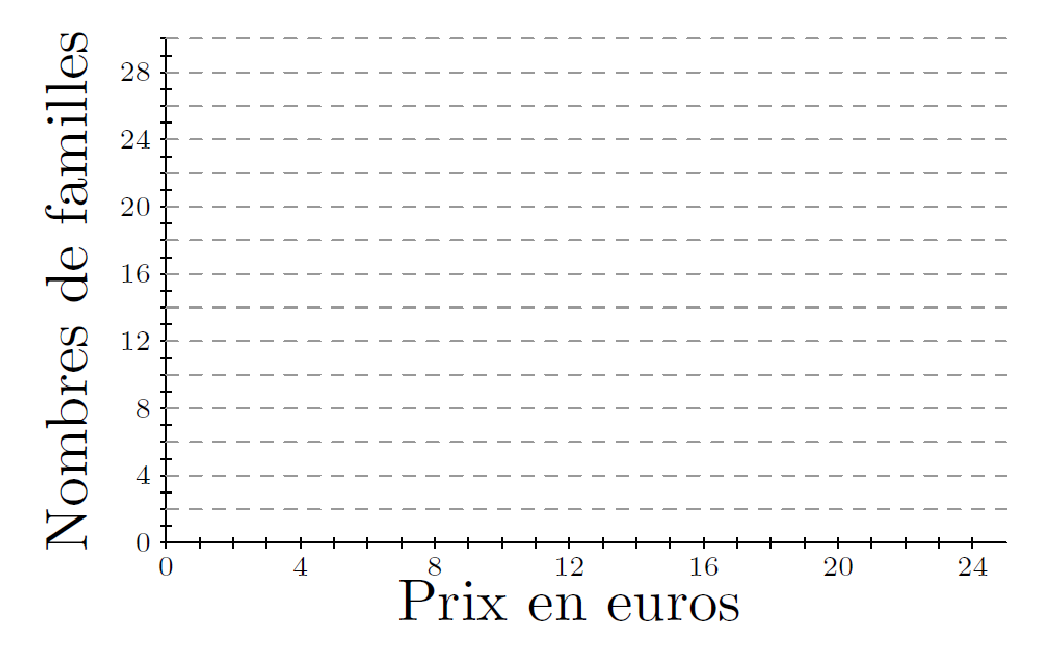
\includegraphics[scale=0.6]{histo2.eps} \\


\exo{}Dans une entreprise, on a étudié l'âge des 125 salariés.
Les résultats de cette étude sont donnés dans le tableau suivant :
\bmul{2}

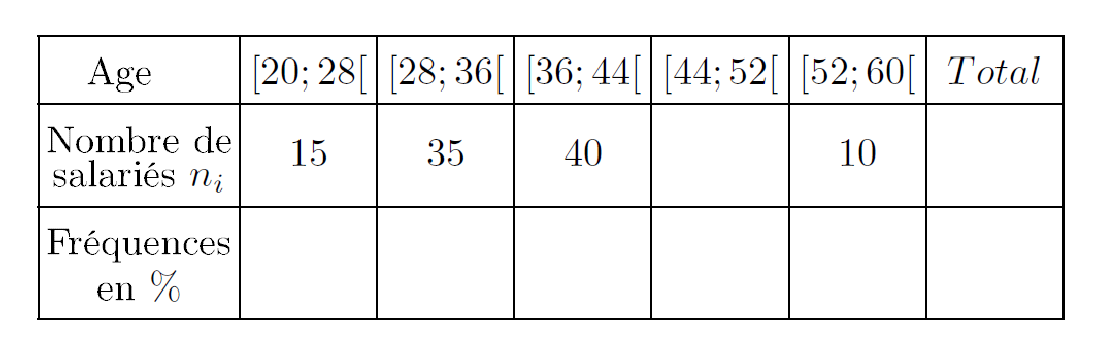
\includegraphics[scale=0.5]{tableau2.eps}\\
\vspace*{0.25cm}
\q Compléter le tableau ci-dessus.\\
\q Tracer l'histogramme des \textbf{effectifs} à l'aide du quadrillage ci-contre.\\ 

\columnbreak
\includegraphics[scale=0.5]{histo3.eps} 
\emul


\q \qa Combien de salariés ont moins de 44 ans?\\
\reponse[3]\\
\qa Combien de salariés ont 36 ans et plus?\\
\reponse[3]\\
\qa Quel pourcentage de salariés a entre 52 ans et 60 ans?\\
\reponse[3]

\end{document}
